\chapter{Layout e interface para usuários}\label{Layout e interface para usuários}\lhead{\leftmark}

\section{Descrição geral da pesquisa de Layout e interface}
A construção do layout e da interface compreendem do desenho à
consolidação da arquitetura geral do sistema. Layout é o desenho, a
identidade visual do sistema; por interface, entende-se o ambiente
através do qual usuários interagem com o sistema. Logo, é na
interface que se implementa a identidade visual, mas além disso, é
na interface que se define a estrutura de navegação e a disposição
das funcionalidades de acordo com o contexto de uso.

A elaboração do layout e da interface não se resumem à mera parte
visual; diz respeito a como usuários interagem com a plataforma,
como funcionalidades e recursos lhes são apresentados, além de
auxiliar na sua navegação por meio de ferramentas auxiliares.

A elaboração do desenho inicial é inicialmente apresentada e
aprovada, e em seguida aprimorada para atender às demandas do
levantamento de funcionalidades.

Em paralelo à evolução do layout, a interface deve ser estruturada
enquanto código, para dar suporte ao desenho. No caso da arquitetura
de sistema adotada, a interface se conecta à uma API, da qual
obtém dados, cabendo à primeira a apresentação dos resultados. Não
cabe à interface lidar com o armazenamento ou a lógica do sistema,
apenas com a lógica da apresentação das informações. Deste modo,
a construção da \emph{API} e a estruturação da plataforma precedem o
desenvolvimento da interface.

Entretanto, por se tratar de uma ferramenta experimental e em fase
de desenvolvimento e maturação, conforme a construção da interface
avançou, foi possível detectar alguns problemas conceituais, além
da incorporação de novas funcionalidades. Logo, na criação do
software Baobáxia, fugiu-se à lógica tradicional de análise de
sistemas compartimentada em fases rígidas. A elaboração do produto
do layout e da interface rendeu sugestões de aprimoramentos na API,
alguns dos quais já implementados, outros anotados para posterior
desenvolvimento.

\section{Levantamento de funcionalidades}
O levantamento das funcionalidades do sistema foi a primeira etapa
realizada para criação do layout e implantação da interface. Para
tal, contamos com levantamentos textuais e na elaboração de um
\emph{wireframe}.

\subsection{Wireframe}
O desenho de wireframe é um método eficiente para o design de
interfaces, ilustrando as páginas dos sistema, suas funcionalidades
e o fluxo de interação entre cada uma delas. Por meio do wireframe
os trabalhos para construção da identidade visual são orientados,
de modo que o desenho seja compatível com a estrutura do sistema.

O wireframe completo está disponível em: \url{https://raw.githubusercontent.com/RedeMocambos/baobaxia/master/doc/layout/wireframe.svg}.
O arquivo pode ser executado utilizando o programa Inkscape \footnote{disponível
  em: \url{http://inkscape.org}.}.

Foram listadas no \emph{wireframe} as seguintes páginas:
\begin{itemize}
  \item login de usuário
  \item home da mucua
  \item visualização da rede
  \item visualização por tag
  \item visualização por tags combinadas
  \item visualização no modo grid
  \item visualização no modo lista
  \item página do arquivo
  \item página do arquivo (visualzada a partir de outra mucua com alta
    conectividade
  \item página do arquivo (visualzada a partir de outra mucua com baixa
    conectividade
  \item envio de arquivos
  \item edição de arquivos
  \item listagem de mucuas
  \item informações da mucua
  \item sincronização de dispositivo
\end{itemize}

Além destas, ainda constam como funcionalidades/ações:
\begin{itemize}
  \item registrar
  \item logout
  \item esqueci a senha
  \item página do mocambola / profile
  \item edição da mucua
  \item lista de requisições da mucua
  \item informações da rede
  \item cabeçalho
  \item rodapé com indicação de uso da mucua
\end{itemize}    

\subsection{Arquitetura}
A arquitetura da interface é modular, conectando-se com a \emph{API}
\footnote{Uma \emph{API}\footnote{Application programming interface}
  especifica um componente de software em termos de suas operações,
  entradas e saídas e coorrespondentes tipos. Seu objetivo é definir
  um conjunto de funcionalidades que são independentes da implementação
  adotada, permitindo que tanto a implementação técnica (para dentro)
  como a interface (que se encaixa) sejam alteradas, sem dano para
  qualquer uma das partes.} do software básico. Isso quer dizer que
é possível desenvolver outras interfaces em cima da mesma \emph{API}
- como uma interface em modo texto, ou uma interface exclusiva para
telefones celulares - sem precisar reprogramar o núcleo do programa.

A arquitetura baseada em \emph{APIs} é perfeitamente adequada para
softwares que se projetam como de longa duração, já que alterações
tanto no interior do sistema como na interface podem ser feitas sem
prejuízo para as outras partes. Uma melhoria interna no núcleo do sistema
pode ser implementada sem que nem sequer se perceba alteração na parte
da interface; do mesmo modo, qualquer alteração e implementação nova da
interface pode ser feita contanto que utilize as rotas da \emph{API}
existente. Trata-se de uma arquitetura modular, desacoplada,
perfeitamente adequada para a natureza de um sistema como o Baobáxia.

A \emph{API} já encontrava-se desenhada e em parte implementada; mas
durante a construção da interface - a parte visual do sistema - novas
tarefas e funcionalidades, expressa em rotas e \emph{urls}, foram
adicionadas, chegando-se a um desenho mais próximo de uma versão
operacional do sistema. 

O desenho da arquitetura da \emph{API} é fundamental para construção
da interface, pois é por meio das urls da \emph{API} que o sistema
irá buscar informações de conteúdo e enviar dados para realizar ações.

As rotas listadas abaixo estão divididas por áreas

\emph{Autenticação}
\begin{itemize}
  \item /login (funcionalidade de login)
  \item /[repo]/[mucua]/login (funcionalidade de login - com caminho)
  \item /logout (funcionalidade de logout)
  \item /[repo]/[mucua]/logout (funcionalidade de login - com caminho)
  \item /register (registro de novos usuários)
  \item /[repo]/[mucua]/register (registro de novos usuários - com caminho)
  \item /lost\_password (recuperação de senha)
  \item /[repo]/[mucua]/lost\_password (recuperação de senha - com caminho) 
\end{itemize}

\emph{Mocambola}
\begin{itemize}
  \item /[repo]/[mucua]/mocambola/[user] {get}          profile do mocambola
  \item /[repo]/[mucua]/mocambola/[user] {put, delete}  edição de dados do mocambola
\end{itemize}

\emph{Mucua}
\begin{itemize}
  \item /[repo]/[mucua] {get}         home da mucua
  \item /[repo]/[mucua] {put}         atualização da mucua
  \item /[repo]/[mucua]/info          informações sobre a mucua
  \item /[repo]/[mucua]/requests      requisições da mucua
\end{itemize}

\emph{Home da rede}
\begin{itemize}                
  \item /rede                         home da rede
  \item /rede/info                    informações da rede
\end{itemize}

\emph{Funcionalidades media}
\begin{itemize}
  \item /[repo]/[mucua]/media {post}                inserir media
  \item /[repo]/[mucua]/media/[uuid] {get}          retornar media
  \item /[repo]/[mucua]/media/[uuid] {put, delete}  atualizar media
  \item /[repo]/[mucua]/media/last {get}            retorna últimas medias adicionadas
  \item /[repo]/[mucua]/media/[uuid]/url            retorna url do arquivo
  \item /[repo]/[mucua]/media/[uuid]/[width]x[height].[format]       retorna imagem da media
  \item /[repo]/[mucua]/media/[uuid]/related        retorna media relacionada à media atual [uuid]
\end{itemize}

\emph{Funcionalidades básicas para definição de escopo}
\begin{itemize}
  \item /repository/list                     lista repositórios disponíveis
  \item /repository/*                        retorna repositório padrão
  \item /[repo]/mucuas                       retorna mucuas do [repositório]
  \item /mucua/                              retorna mucua padrão
  \item /mucua/list                          retorna lista das mucuas
\end{itemize}

\emph{Busca}
\begin{itemize}
  \item /[repo]/[mucua]/bbx/search/[arg1]/[arg2]/...  busca por argumentos
\end{itemize}

\section{Layout da interface}
Por Layout entendemos o desenho propriamente dito, na forma de uma
imagem, a ser implementada pelo programador web. O trabalho divide-se
entre a criação de uma identidade visual (ideia) e o desenho das
telas principais (a aplicação da ideia a casos reais).

\subsection{Identidade visual}

Foi criada uma logomarca para o Baobáxia, considerando ...


\begin{figure}[htbp]
  \centering
  
\includegraphics[width=\textwidth]{./Fig/Logo_BBX.pdf}
  \rule{35em}{0.5pt}
  \caption[Logomarca Baobáxia]{Logomarca Baobáxia}
  \label{fig:Logo_BBX}
\end{figure}

\begin{figure}[htbp]
  \centering
  
\includegraphics[width=\textwidth]{./Fig/Logo_BBX_Na_Rota.pdf}
  \rule{35em}{0.5pt}
  \caption[Logomarca Baobáxia na Rota dos Baobás]{
    Logomarca Baobáxia na Rota dos Baobás}
  \label{fig:Logo_BBX_Na_Rota}
\end{figure}

\subsection{Desenho das telas principais}

Após elaborada a identidade visual, partiu-se para o desenho das
principais telas do sistema. A partir delas, o trabalho de codificação
da interface pode ser iniciado, e também ajustes no desenho puderam ser
feitos após a implementação em código do desenho.

Decidiu-se que as principais telas para a fase inicial do projeto seriam:
\begin{itemize}
  \item Página inicial / tela de login
  \item Página inicial da mucua
  \item Página inicial da rede
  \item Rodapé com indicativos sobre utilização da mucua
  \item Interface de busca combinada
  \item Página do conteúdo
\end{itemize}

\begin{figure}[htbp]
  \centering
  
\includegraphics[width=\textwidth]{./Fig/layout-login.pdf}
  \rule{35em}{0.5pt}
  \caption[Página de login]{Página de login}
  \label{fig:layout-login}
\end{figure}

\begin{figure}[htbp]
  \centering
  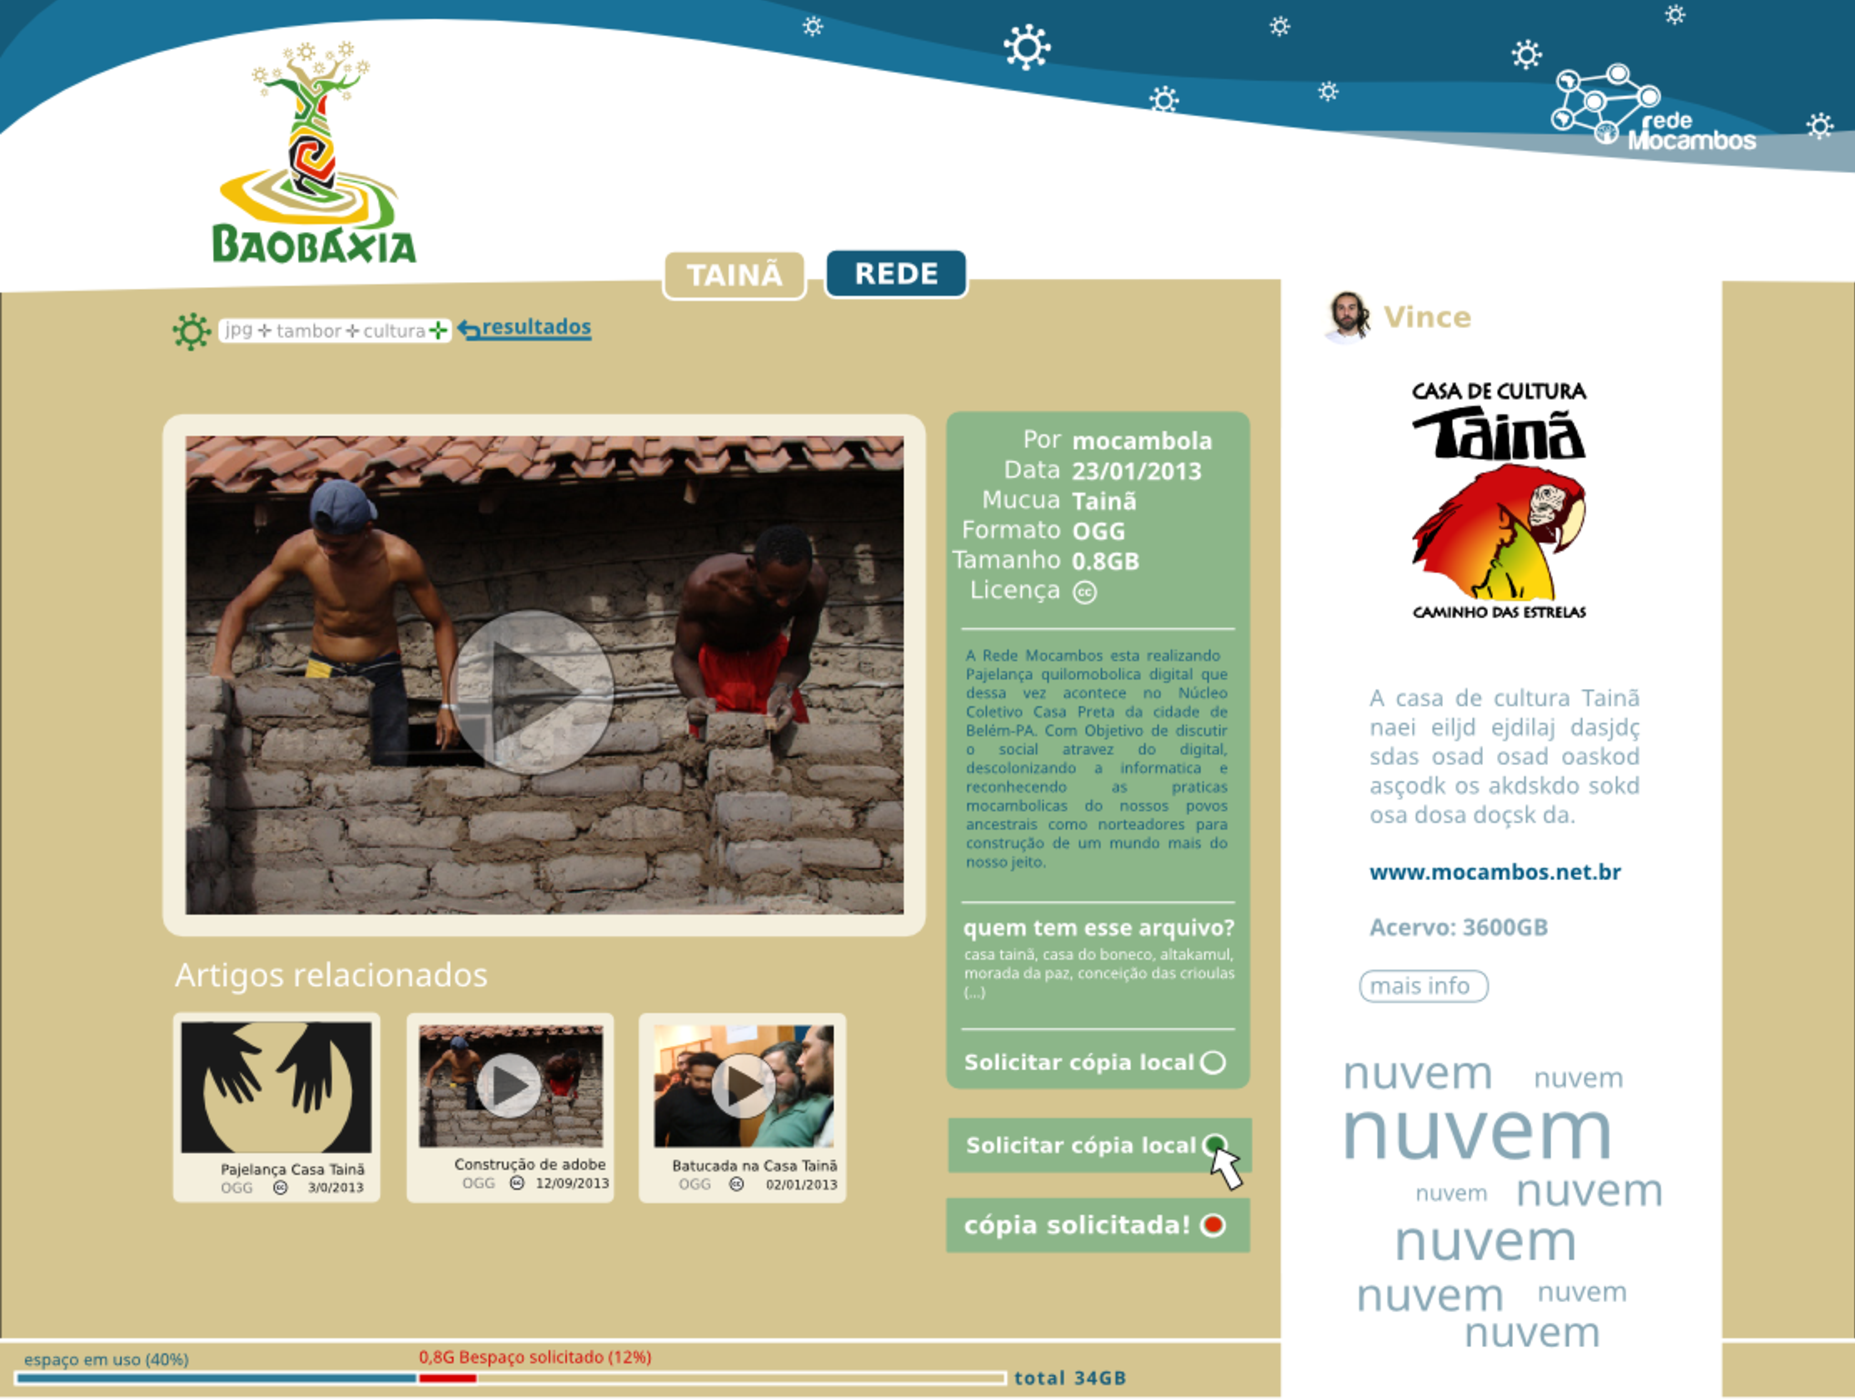
\includegraphics[width=\textwidth]{./Fig/layout-pgCONTEUDO.pdf}
  \rule{35em}{0.5pt}
  \caption[Página do conteúdo]{Página do conteúdo}
  \label{fig:layout-pgCONTEUDO}
\end{figure}

\begin{figure}[htbp]
  \centering
  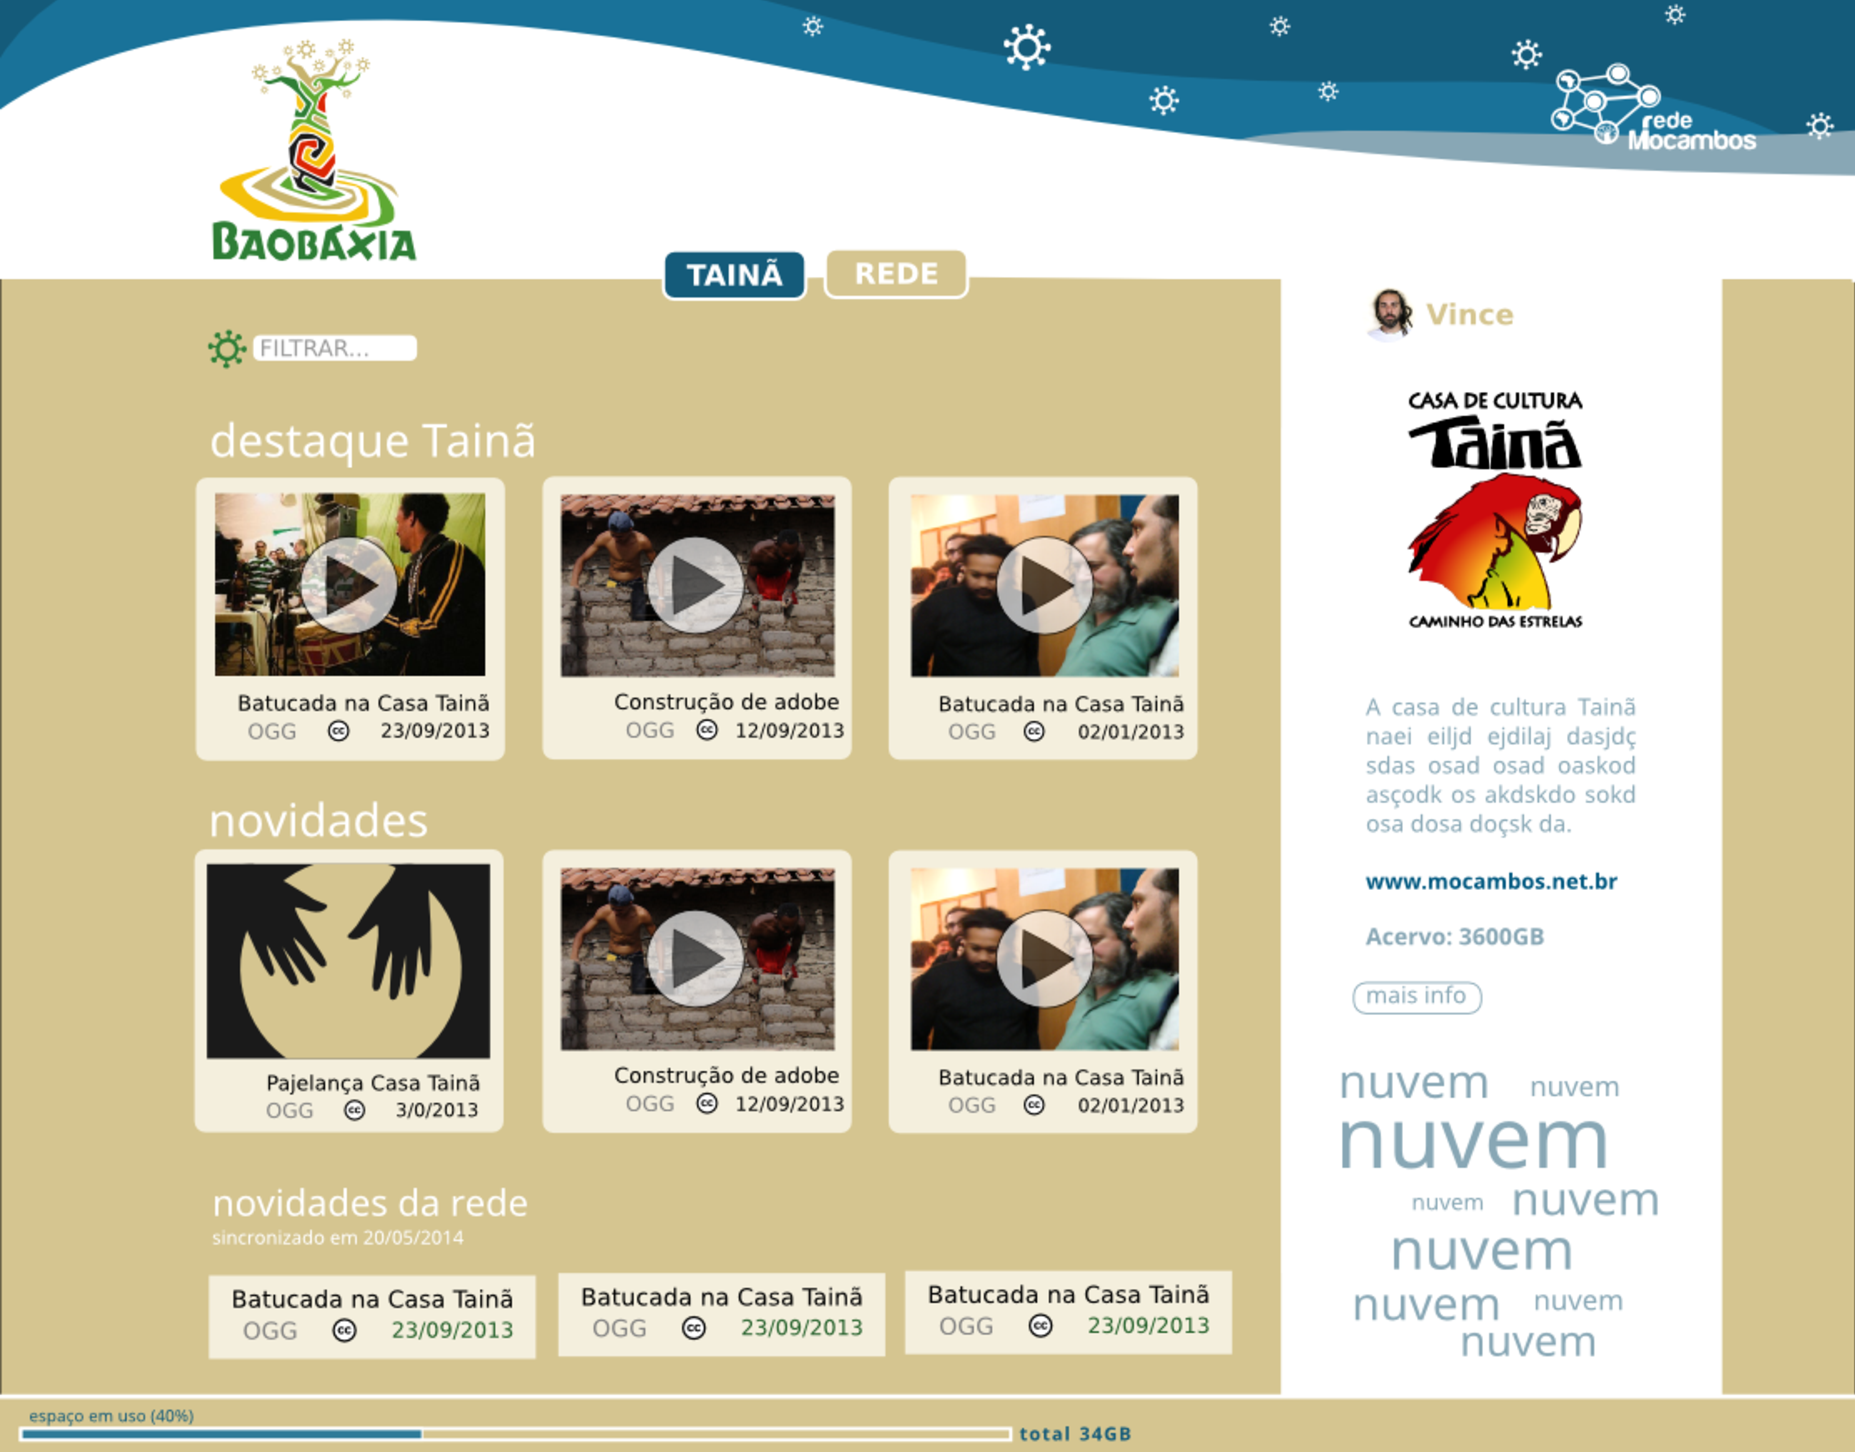
\includegraphics[width=\textwidth]{./Fig/layout-pgMUCUA.pdf}
  \rule{35em}{0.5pt}
  \caption[Página da Mucua]{Página da Mucua}
  \label{fig:layout-pgMUCUA}
\end{figure}

\begin{figure}[htbp]
  \centering
  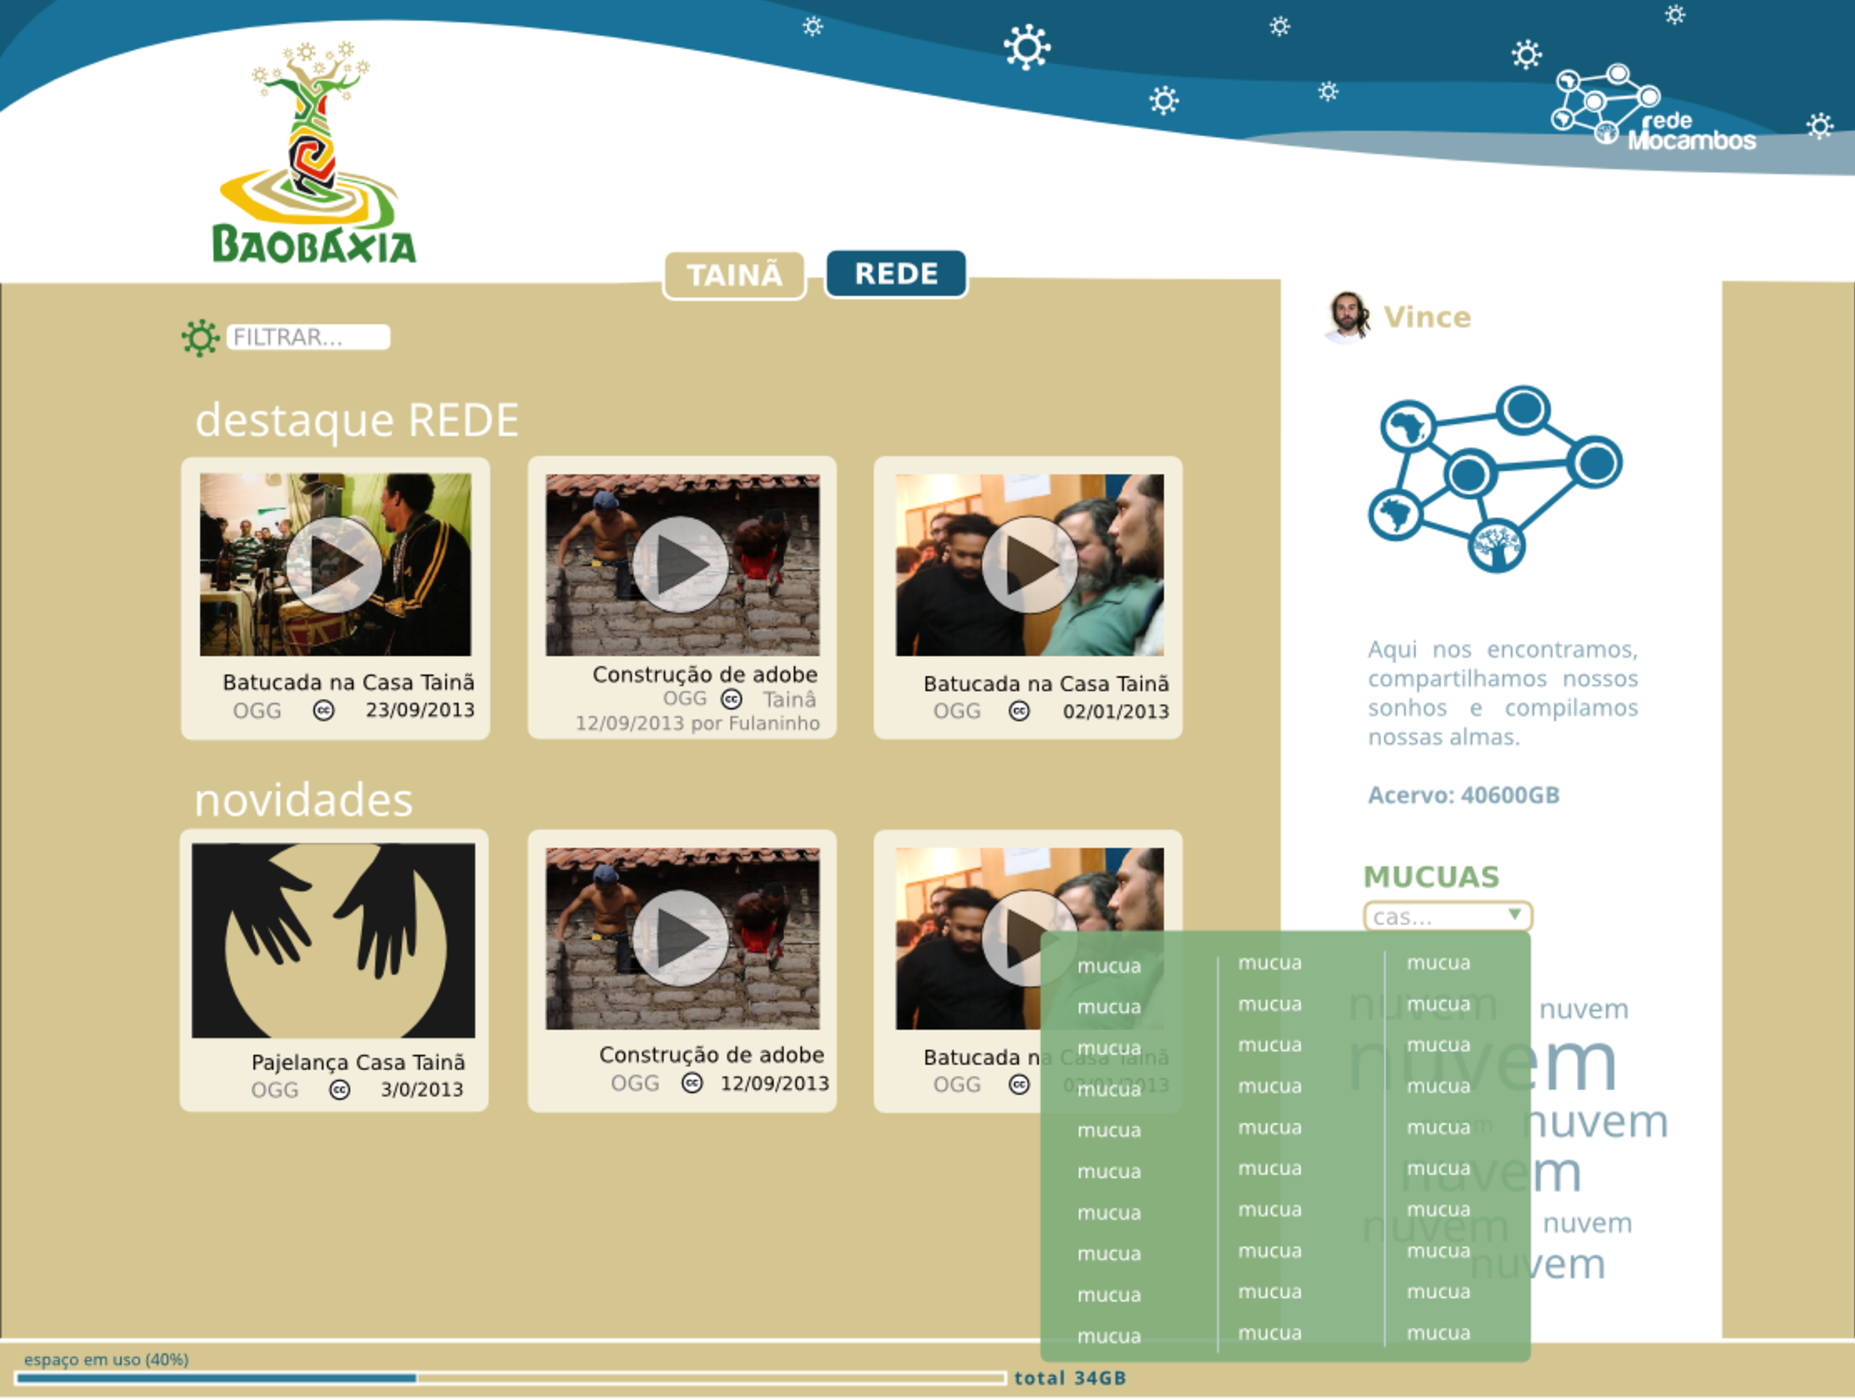
\includegraphics[width=\textwidth]{./Fig/layout-pgREDE.pdf}
  \rule{35em}{0.5pt}
  \caption[Página da Rede]{Página da Rede}
  \label{fig:layout-pgREDE}
\end{figure}

\begin{figure}[htbp]
  \centering
  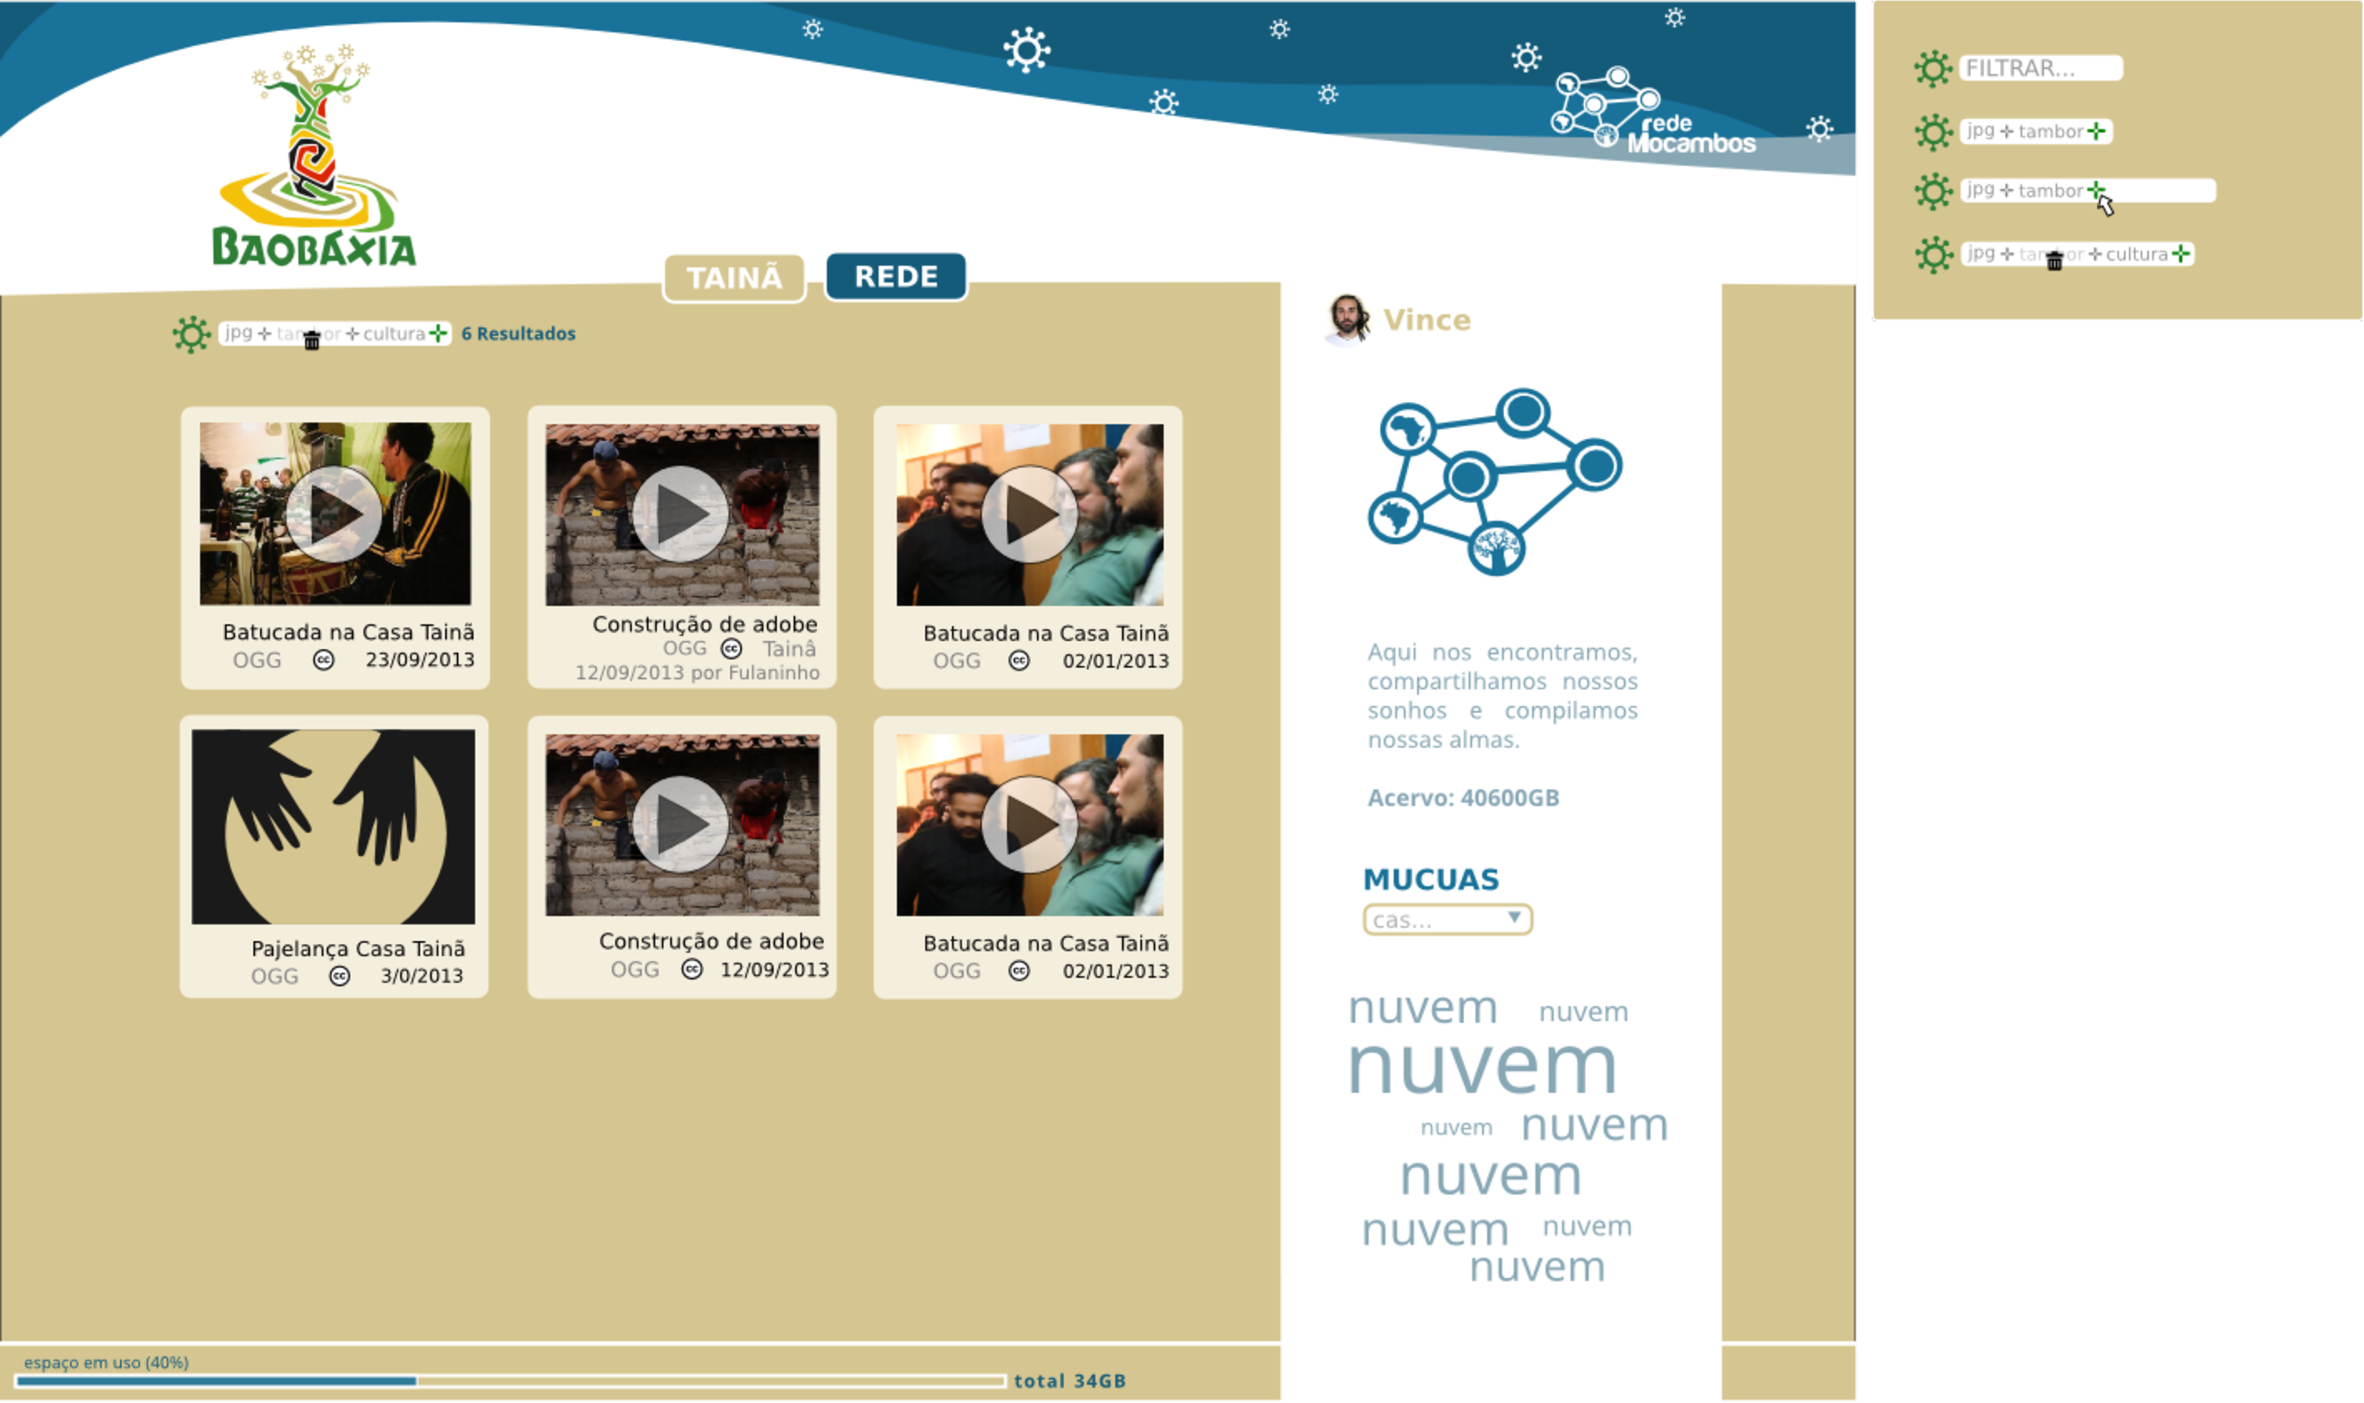
\includegraphics[width=\textwidth]{./Fig/layout-pgREDEbusca.pdf}
  \rule{35em}{0.5pt}
  \caption[Página da Rede com busca]{Página da Rede com busca}
  \label{fig:layout-pgREDEbusca}
\end{figure}

\section{Interface para usuários}
A interface propriamente dita é a interação do sistema com o usuário;
deve conter as funcionalidades básicas do sistema disponíveis para
interação, implementada na forma de uma página de internet. O presente
tópico pretende discorrer sobre as tecnologias e a arquitetura adotadas.

\subsection{Arquitetura da interface}
A interface do Baobáxia é a parte superior, mais aparente, do sistema,
conversando com o seu núcleo por meio de uma \emph{API}. Decidiu-se
pela implementação de uma interface em HTML e JavaScript, utilizando
uma série de bibliotecas de código, buscando separar as camadas do modelo
de dados, lógica de programação, roteamento, visualização dos dados e
templates de páginas.

Para garantir tal arquitetura, adotamos as seguintes bibliotecas:
\begin{itemize}
  \item \emph{Backbone.Js}: para lidar com o modelo de dados e as conexões
    com a \emph{API}, cuidando da atualização dos dados
  \item \emph{Require.js}: cuida do carregamento dinâmico das bibliotecas
    e suas dependências, adicionando tal funcionalidade ao JavaScript
  \item \emph{Underscore.js}: biblioteca assistente para o código, adiciona
    uma série de métodos úteis ao trato com os dados e a exibição dos
    conteúdos na forma de Templates
  \item \emph{Jquery} e outras bibliotecas auxiliares de código, para
    manipulação dos dados do \emph{DOM} \footnote Document Object Model
\end

\subsection{Implementação da interface junto à API}
Foi montada uma estrutura que permite a fácil e rápida expansão das
funcionalidades do sistema na interface, obedecendo a um padrão de rotas e
disposição de funcionalidades. A interface se montou acompanhando a \emph{API},
surgerindo novas funcionalidades ainda não implementadas no núcleo do sistema.

A estrutura é a que segue:
\begin{itemize}
  \item definição de bibliotecas e mapeamento de endereços
  \item funcionalidades relacionadas à media
  \item funcionalidades relacionadas à tarefas do Baobáxia
  \item visualizações (autenticação, media, mocambola, mucua e comuns)
  \item templates (modelos de dados para autenticação, media, mocambola e mucua)
  \item estilos (formatação HTML / arquivos css)
\end{itemize}

\subsection{Implementação das telas principais}
Foram implementadas as telas de login com funcionalidade de logout,
página inicial da mucua com listagem de conteúdos da mucua e dados da mucua,
página inicial da rede com listagem de conteúdos de toda a rede (apenas
metadados), página do conteúdo, página de edição do conteúdo, página de
inserção de conteúdos, listagem de conteúdos por mocambolas, navegação
por categorias, listagem em lista ou em grid.
